\svnidlong
{$LastChangedBy$}
{$LastChangedRevision$}
{$LastChangedDate$}
{$HeadURL$}

\chapter{Introduction}
\label{ch:intro}
%Author: \svnauthor; Revision: \svnrev; Last changed on: \svndate; URL: \url{\svnkw{HeadURL}}

The present chapter is a review of the scientific literature in order to introduce the concepts that form the background and the frame of the present thesis. For a more concise presentation of this work, its standpoints and its goals, see the \nameref{ch:abstract}.

In \SectionRef{sec:glass_transition} we will introduce the basic phenomenology and terminology of the glass transition. This will set the path for \SectionRef{sec:sc_dynamics} and the dynamics of supercooled liquids. \SectionRef{sec:static_cause} will focus on the open question of the relationship between structure and dynamics in the supercooled liquids. The main goal of this work will to try to answer to this question. Finally \SectionRef{sec:HS-colloids} will present the physics of the particular system we studied: colloidal hard spheres.

\section{Glass transition}
\label{sec:glass_transition}
When we lower the temperature of a liquid, at some point we meet a first order phase transition to the crystal. Yet, under certain conditions it is possible to avoid crystallisation and to obtain a metastable phase called a supercooled liquid. When the temperature is decreased even lower, the dynamics slows down dramatically until we are unable to equilibrate the system within reasonable experimental times. The system has become a non-crystalline solid: a glass. \FigureRef{fig:cooling} summarise this process.

\begin{figure}
	\centering
	\def\svgwidth{0.8\textwidth}
   	\input{cooling.pdf_tex}
	\caption{Schematic representation of the entropy as a function of temperature in a liquid, from the high-temperature phase, down to the deeply supercooled phase. All the relevant temperatures are marked. Above each temperature we report the approximate value (in seconds) of the relaxation time. The cooling curves in different colours corresponds to different cooling rates and thus to slightly different temperatures where the system falls out of equilibrium.
	From \ReferenceRef{cavagna2009supercooled}}
	\label{fig:cooling}
\end{figure}

\subsection{From liquid to solid}
\label{sec:liquid_solid}

The distinction between a solid and a liquid does not involve thermodynamics but pure mechanics. A solid is defined as a material that does not flow; if we apply a constant stress on a solid, the strain stays constant in time. On the contrary, a liquid flows; if we apply a constant stress on a liquid, the strain decays with time. We made here no assumption about the structure of the material or the state point of the system, in equilibrium or not, metastable or not. However, this distinction depends on the time-scale: the stress does not relax instantaneously in a liquid, but with a characteristic relaxation time $\tau_R$. For times much smaller than $\tau_R$, the liquid has a non-zero elastic response.

For high temperature molecular liquids $\tau_R$ is typically of the order of \unit{10^{-13}}{\second}. However when a liquid approaches the glass transition its characteristic relaxation time increases by many orders of magnitudes. The (kinetic) glass transition temperature $T_g$ is defined as the temperature where $\tau_R$ exceed the experimentally accessible time scale (often \unit{\sim 10^3}{\second}). The system cannot relax; it has become a solid. As you can see, $T_g$ is not a well-defined thermodynamic temperature, but depends on experimental contingencies as the patience of the experimentalist and also the cooling rate.

If the glass transition is continuous and its temperature not well-defined thermodynamically, why is it called a \emph{transition}? It is because the slowing down of the system is dramatic near $T_g$; $\tau_R$ increases by orders of magnitudes over a few Kelvins. Moreover in many systems the increase of the relaxation time is so sharp that actually the position of $T_g$ hardly moves even with a substantial change in the cooling rate. That is because near $T_g$ the temperature dependence of the relaxation time follows at least the Arrhenius law and is often fitted by the empirical \ac{VFT} relation~\citep{Vogel1921, Fulcher1925, Tammann1926}
\begin{equation}
	\tau = \tau_0 \exp{\left(\mathcal{D}\frac{T_0}{T_0-T}\right)}
	\label{eq:VFT}
\end{equation}
where $\mathcal{D}$ is called the fragility and is characteristic of the glass-former. $T_0$ is a temperature below the kinetic $T_g$ where the relaxation time would diverge. If there is some thermodynamic transition behind the dynamical arrest, $T_0$ is a good candidate for the transition temperature. That is why $T_0$ is often called the ideal glass transition temperature.

\subsection{Configuration and vibration}
\label{sec:config_vib}

A thermodynamic interpretation of the glass transition was proposed by \citet{Goldstein1969}. His idea is to look at the energy landscape of the system in the phase space, i.e. the space of all the configurational degrees of freedom. For example, for a monatomic liquid in three dimensions, this is the space of all $3 N$ coordinates of the particles. This energy landscape has many local energy minima that represents the metastable configurations of the system. The absolute minima is the crystal. When the temperature is lowered rapidly enough, the system gets stuck in one of these local minima, vibrating in its potential well. The system has only one possible configuration, it cannot rearrange or flow: it has become a solid. With Goldstein's picture in mind, one can write the entropy $S$ of a low temperature system as the sum of a configurational part and a vibrational part.
\begin{equation}
	S = S_c + S_{vib}
	\label{eq:config_vib}
\end{equation}

A liquid explores the configuration space and thus has a high configurational entropy $S_c$. A solid is limited to one configuration and its entropy is only vibrational. For a more formal approach to this splitting, see~\citep{Scheidler2001, Nielsen1999}. The loss of configurational entropy at the glass transition was put into light by measurements of the constant pressure specific heat $C_P$~\citep{ANGELL1988}. The sharp drop sketched in \FigureRef{fig:specific_heat} indicates that the dynamical arrest suddenly cuts the degrees of freedom accessible to the system. Moreover, the values of $C_P$ for the glass and for the crystal are very close. This indicates that as in a crystal, the only degrees of freedom accessible to the glass are the vibrations of the particles around their mean position.

\begin{figure}
	\centering
	\def\svgwidth{0.8\textwidth}
   	\input{specific_heat.pdf_tex}
	\caption{Schematic view of the specific heat temperature dependence at the dynamic glass transition. The specific heat drops at the dynamic glass transition to approximately the same value it has in the crystal phase. This is because below $T_g$ we are not giving the system enough time to be ergodic. Roughly speaking, a glass is stuck in a single potential energy minimum for a long time, so that it loses all the configurational degrees of freedom. From \ReferenceRef{cavagna2009supercooled}}
	\label{fig:specific_heat}
\end{figure}

\subsection{Two types of solids}
\label{sec:X+glass}

As the crystal, the glass is non-ergodic. But contrary to the crystal, the glass is intrinsically out of equilibrium. Even though one-time quantities (as the volume or the energy) may look almost constant in the long time limit, two-time quantities (as the dynamic correlation function) show a stark off-equilibrium behaviour, in that they depend explicitly on both times, rather than on their difference. In other words, the properties of the system depend on the time elapsed from the instant the system was cooled below $T_g$. This phenomenon is called ageing and lies beyond the scope of this thesis.

The particles of a crystal are vibrating around positions that form a periodic lattice, whereas a glass present no hint of positional order. The static structure of the particles in a supercooled liquid close to $T_g$, and even in a glass below $T_g$, is virtually indistinguishable from that of a liquid at temperatures well above $T_g$. As far as structure is concerned, a glass looks exactly the same as a liquid~\citep{Ernst1991, Leheny1996, PRICE1987, vanblaaderen1995rss}. Here the indicator of structure is a static two body density correlator like the \ac{Sq}, which is usually very good at detecting the difference between phases. In general, the relaxation time $\tau_R$ increases by 12-14 orders of magnitude at $T_g$. Yet, when this happens the structure does not show anything much more relevant going on than what is shown in \FigureRef{fig:rdf_glass}. We conclude that it is impossible to use the structure factor, or any other standard structural quantity, to understand whether or not the sample is close to the glass transition, is still a supercooled liquid or has become a glass.

\begin{figure}
	\centering
	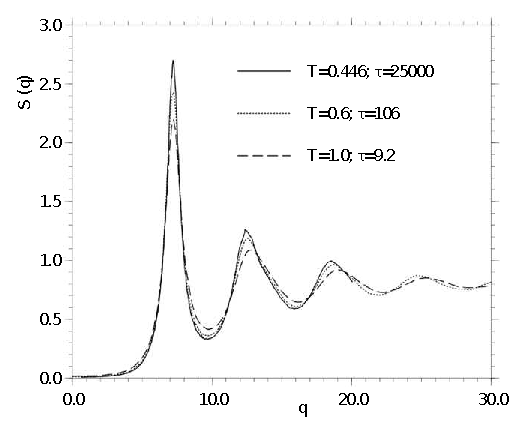
\includegraphics[width=0.8\textwidth]{sq_kob}
	\caption{The static structure factor $S(q)$ in a Lennard-Jones liquid at three different temperatures. The relaxation time $\tau_R$ increases by almost 4 orders of magnitude, and yet the structure factor shows no particular change. (from \citep{Kob2002})}
	\label{fig:rdf_glass}
\end{figure}

%\begin{figure}
%	\centering
%	\includegraphics[width=0.8\textwidth]{kawasaki_rdf}
%	\caption{$\phi$-dependence of the radial distribution function g(r) for $\Delta = 0\%$ and $\Delta = 6\%$. The blue colour means disordered, whereas the red colour means ordered. Comparison of left and right tells us that there is no disorder–order transition for $\Delta = 6\%$. However, we can see the splitting of the second peak at high $\phi$ even for $\Delta = 6\%$ (see the arrows), indicating the possible existence of medium-range order.}
%	\label{fig:rdf_glass}
%\end{figure}

\subsection{Glass or supercooled?}
\label{sec:glass_or_sc}
Following \citet{cavagna2009supercooled}, let us make here a clear semantic distinction. The glass is fundamentally out of equilibrium, whereas the supercooled liquid is in a metastable equilibrium.

The supercooled liquid is by definition metastable to the crystal. However, we can experimentally equilibrate a liquid in its metastable phase, in such a way that time-translation invariance (and thus the dynamical fluctuation dissipation theorem) holds. In such situation, no experimental measurement is able to tell us that the system is metastable. Only an explicit crystallization of the sample would unveil metastability. Therefore, with a slight abuse of language, we will call this the \emph{equilibrium} liquid phase, supercooled or not depending on whether we are below or above the melting temperature. As always in first-order phase transitions, there is no way to experimentally detect the presence of the transition temperature, as long as the system remains equilibrated into one of the two phases.

As we have seen before, the time translation invariance does not hold below $T_g$. We will use the noun "glass" and the adjective "glassy" to design the out of equilibrium solid resulting of the dynamical arrest and its phenomenology, like ageing.

%
%\begin{description}
%	\item[$T_m$] The melting point, where a first-order phase transition between liquid and crystal occurs;
%	\item[$T_c$] Goldstein's crossover temperature from a high-T nonactivated dynamics to a low-T activated one;
%	\item[$T_g$] The dynamic glass transition, where the relaxation time exceeds the conventional experimental time of \unit{10^3}{\second}, the longer the available experimental time, the lower the temperature where the system falls out of equilibrium forming a glass;
%	\item[$T_K$] Kauzmann's entropy crisis temperature, where the extrapolated liquid entropy hits the crystal entropy, and where according to some theories there is a thermodynamic phase transition;
%	\item[$T_0$] The temperature where the \ac{VFT} fit locates a divergence of the relaxation time. Often identified with $T_K$
%\end{description}

\section{Supercooled liquid dynamics}
\label{sec:sc_dynamics}

\subsection{Dynamic quantities}
\label{sec:isf_msd}

To define the dynamics of a time-dependent quantity $a(t)$, we need to measure it at two times: $t_0$ and $t_0+t$. For instance, a displacement is defined as the difference in position of the same object at two different times. 
\begin{equation}
	\Delta \vec{r}(t_0, t) = \vec{r}(t_0+t) - \vec{r}(t_0)
	\label{eq:displacement}
\end{equation}
with $\vec{r}(t0)$ the vector position of the object at time $t_0$.

In a statistical system, we often need to define an ensemble averaged dynamic correlation function:
\begin{equation}
	\mathcal{C}(a)(t_0, t) \equiv \left\langle a(t_0) \cdot a(t_0+t) \right\rangle
	\label{eq:correlation}
\end{equation}

If we deal with a statistical mechanic system at equilibrium, the ensemble average of the dynamic quantity should not depend on $t_0$, but still depend on the time lag $t$. However, one must keep in mind that $t$ is a difference between times, and not an absolute time. 

Until now, we used the relaxation time $\tau_R$ or the viscosity $\eta$ as our dynamical variable. We could have used equivalently the diffusion constant $D$. The common point of all these quantity is that they correspond to the integral of dynamical functions over all the (accessible) time lags. For instance, the relaxation time at the wavevector $q$, \latin{i.e.} at a scale $\sim \pi/q$, is the integral of the self \ac{ISF}:
\begin{equation}
	F_s(q,t) \equiv \frac{1}{N} \Bigl\langle\sum_{i=1}^N e^{-\imath\vec{q}\cdot\bigl(\vec{r_i}(t)-\vec{r_i}(0)\bigr)}\Bigr\rangle
	\label{eq:isf}
\end{equation}
where we recognise a time correlation function. The corresponding observable is $\exp{\left(\imath\vec{q} \cdot \vec{r_i}(t)\right)}$, the Fourier transform of the density fluctuations of the particle $i$. In an ergodic system, the self \ac{ISF} should decay to $0$ with a characteristic time equal to $\tau_R$, but not in a solid (crystal or glass) where it saturates at a finite value.

Another useful function, in real space this time, is the \ac{MSD}:
\begin{equation}
	\Delta r(t)^2 = \left\langle\| \vec{r_i}(t)-\vec{r_i}(0)\|^2\right\rangle
	\label{eq:msd}
\end{equation}

At very short times, the trajectory of the particles is ballistic: the particles do not influence each-other. We have $\Delta r(t)^2 \sim t^2$. In a solid the \ac{MSD} saturates to a constant value that corresponds to the amplitude of the vibration of the particles. In a liquid the particles diffuse, so at long times we have $\Delta r(t)^2 \sim D t$.

\subsection{Two step relaxation}
\label{sec:2steps}

\begin{figure}
	\centering
	\subfloat
		[Self \acs{ISF} evaluated at the value of q where the static structure factor has the main peak. At high temperatures the decay is exponential, but when the temperature get close to $T_g$ a plateau is formed and relaxation proceeds in two steps. Source \citep{Kob1995}]
		{\label{fig:isf_kob}\def\svgwidth{0.5\textwidth}\input{isf_kob.pdf_tex}}
	\subfloat
		[The \acs{MSD}. At high temperature there is a crossover from ballistic transport to diffusion. At low temperatures this crossover is interrupted by a plateau similar to what happens for the self \acs{ISF}. Source \cite{kob1995tmc}]
		{\label{fig:msd_kob}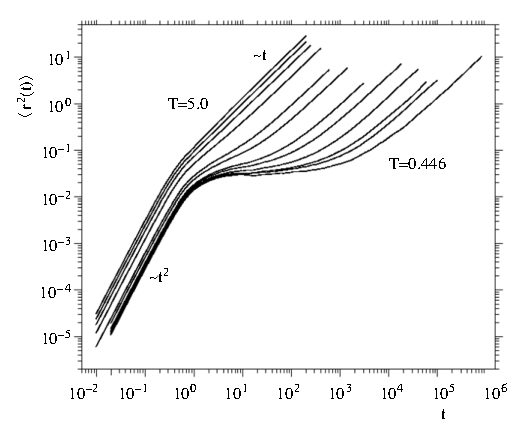
\includegraphics[width=0.5\textwidth]{msd_kob}}
	\caption{Typical dynamics of a supercooled liquid, here a binary Lennard-Jones system. Note that the time scales are logarithmic.}
	\label{fig:dynamics_kob}
\end{figure}

At high temperatures, the self \ac{ISF} decays exponentially. \FigureRef{fig:isf_kob} shows how this behaviour changes with supercooling. When decreasing the temperature a plateau appears in the correlation function that stretch to longer and longer times when approaching the glass transition. We can define two relaxation processes:
\begin{description}
	\item[The $\beta$-relaxation] appends at short times and leads to the plateau.
	\item[The $\alpha$-relaxation] is the decay from the plateau at long times.
\end{description}

The two step relaxation process is the signature of the supercooled liquid dynamics. When a plateau appears in a dynamic correlation function, a glass transition is near. We have an equilibrium measurement that informs us about the glass transition. This means that the glass transition is a physically meaningful concept.

The $\beta$-relaxation does not depend much on the temperature: the plateau is reached in comparable times at shallow and deep supercooling. However the time needed to leave the plateau gets longer by orders of magnitude and is the main cause of the divergence of the relaxation time $\tau_R$.

Obviously, the relaxation of the system cannot be described by a single relaxation time. In a first approximation, we can define a $\tau_\beta$ and a $\tau_\alpha$. The latter is the dominant relaxation time of supercooled fluids. From now on, we will use the expression "relaxation time" indifferently about $\tau_R$ at high temperature or $\tau_\alpha$ when the two step relaxation can be defined.


\subsection{Cage theory}
\label{sec:cage}

To understand more easily what the two step relaxation means in real space, we can have a look a the \ac{MSD} (see \FigureRef{fig:msd_kob}). At high temperature, we have a smooth transition between a ballistic regime where $\Delta r(t)^2 \sim t^2$ and a diffusion regime where $\Delta r(t)^2 \sim t$. The displacement corresponding to this transition is the mean free path of the particles, \latin{i.e.} the distance a particle can go without colliding with an other.

At lower temperatures, we see once again a plateau that intercalates just between the two regimes. The particle has encountered many collisions but does not diffuse. If we look at the actual value of the \ac{MSD} in correspondence of the plateau, we discover that it is quite small, well below the (square) inter-particle distance~\citep{kob1995tmc} and does not evolve much with temperature.

From theses facts emerges a quite simple picture: the particle cannot diffuse because it is always colliding into its neighbours. It is like the particle was trapped in a \emph{cage} formed by its neighbours. The plateau corresponds to the time passed in the cage. At long time the particle eventually escapes its cage and the diffusion behaviour is recovered. Don't forget that the time is in logarithmic scale: after the particle has got out of the cage, it is effectively out of any cage.

\begin{figure}
	\centering
	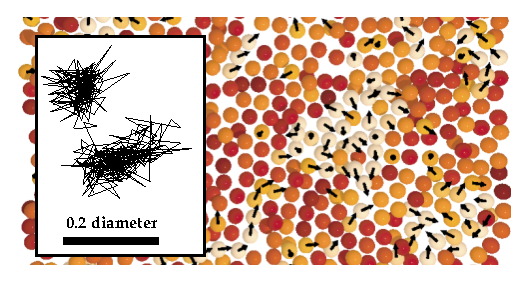
\includegraphics[width=\textwidth]{cage_weeks}
	\caption{A cut through a three-dimensional hard sphere colloidal supercooled liquid observed by confocal microscopy. The arrows indicate the direction of motion for particles with displacements superior to a tenth of diameter during a time corresponding to the middle of the plateau. The arrows are all the same length in three dimensions, so shortened arrows indicate motion in or out of the picture. Lighter colours indicate particles with larger displacements. Inset: A trajectory of one particle from this sample exhibiting cage hopping. Source \citep{weeks2002pcr}}
	\label{fig:cage_weeks}
\end{figure}

This phenomenon was observed experimentally at the microscopic level by the same sort of techniques we will be using is this thesis (see \ChapterRef{ch:Experimental} and \ChapterRef{ch:tracking}). As displayed in \FigureRef{fig:cage_weeks}, \citet{weeks2002pcr} observed indeed the particles rattling in their cages. The displacement due to a single hoping process between cages proved to be only a fraction of the inter-particle distance.

The cage theory can be mapped back to the correlation function: the $\beta$-relaxation is interpreted as the motion between two collision with the neighbours; the plateau indicates that the particle position does not decorrelate further during all the time spent in the cage; the $\alpha$-relaxation corresponds to the escape from the cage and the recovery of ergodicity.

However useful is the picture of the cage to describe what happens in supercooled liquid, it is neither explicative nor complete. We don't know why the neighbours begin to form cages when supercooling the system, and why the frequency of cage hopping decreases at least exponentially with temperature when approaching $T_g$. Furthermore, the right picture is maybe not a particle breaking its cage but a group of particles rearranging cooperatively~\citep{Kob1997, Donati1998, Donati1999, kegel2000swe, Perera1999, weeks2000, weeks2002pcr} as suggested by the clusters and strings of moving particles displayed in \FigureRef{fig:cage_weeks}.

\subsection{Non-Gaussian distribution of the dynamics}
\label{sec:nongaussian}

The major drawback of the cage picture is that it considers all particles as equivalent, diffusing independently at the same rate. If this picture was true, the distribution of the displacements should be Gaussian. This proves to be wrong, as displayed in \FigureRef{fig:not_gaussian}.

\begin{figure}
	\centering
	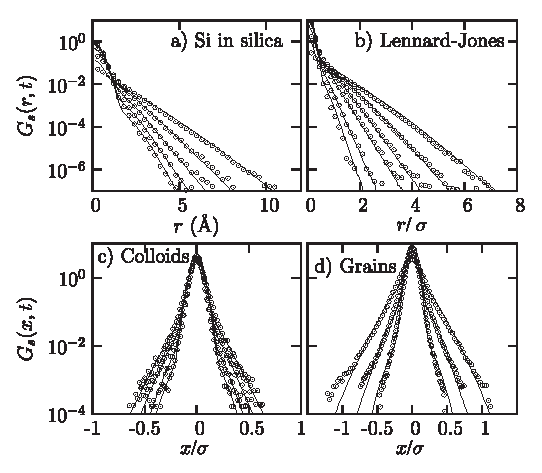
\includegraphics[width=0.8\textwidth]{not_gaussian}
	\caption{Time evolution of the distribution of the displacements for silicon atoms in silica, Lennard-Jones particles, hard-sphere colloids, and grains (open circles), fitted with a combination of a Gaussian for the central part and broad exponential tails (full lines). From~\citep{Chaudhuri2007}}
	\label{fig:not_gaussian}
\end{figure}

The distribution of the displacements is not Gaussian, it has fat exponential tails for large displacement. This is interpreted as the existence of two distinct populations of particles: localized particles that contribute to the central Gaussian distribution and mobile particles that contribute to the exponential tails. A particle that was able to jump out of its cage recently is much more likely to jump again than a particle that has been localised for some time. Jumping evens are not independent.

To quantify such a non-gaussianity of a distribution, the relevant quantity is its (reduced, normalized) fourth moment, the kurtosis often called the \ac{NGP}. In the case of the displacement, it is expressed from the mean square and mean quadratic displacements
\begin{equation}
	\alpha_2(t) \equiv \frac{3 \left\langle {\Delta r}^4(t) \right\rangle}{5 {\left\langle {\Delta r}^2(t) \right\rangle}^2}-1
	\label{eq:ngp}
\end{equation}
Once again, $t$ is a time difference from an arbitrary reference time $t_0$. This function has a more and more pronounced bell shape when approaching the glass transition (see \FigureRef{fig:ngp_kob}). The \ac{NGP} starts to increase on the time scale of the $\beta$-relaxation, reaches its maximum and starts to decrease on the time scale of the $\alpha$-relaxation. The maximum of the \ac{NGP} corresponds to the end of the plateau and appends at later and later times with decreasing temperature.

The decrease to zero of the \ac{NGP} at long times is physically meaningful: the distinction between mobile and localised particles is only transient. If we integrate the displacements over long enough time, all the particles are alternatively localised and mobile.

\begin{figure}
	\centering
	\subfloat
		[\acl{NGP} function of time with increasing supercooling. From~\citep{Kob1997}.]
		{\label{fig:ngp_kob}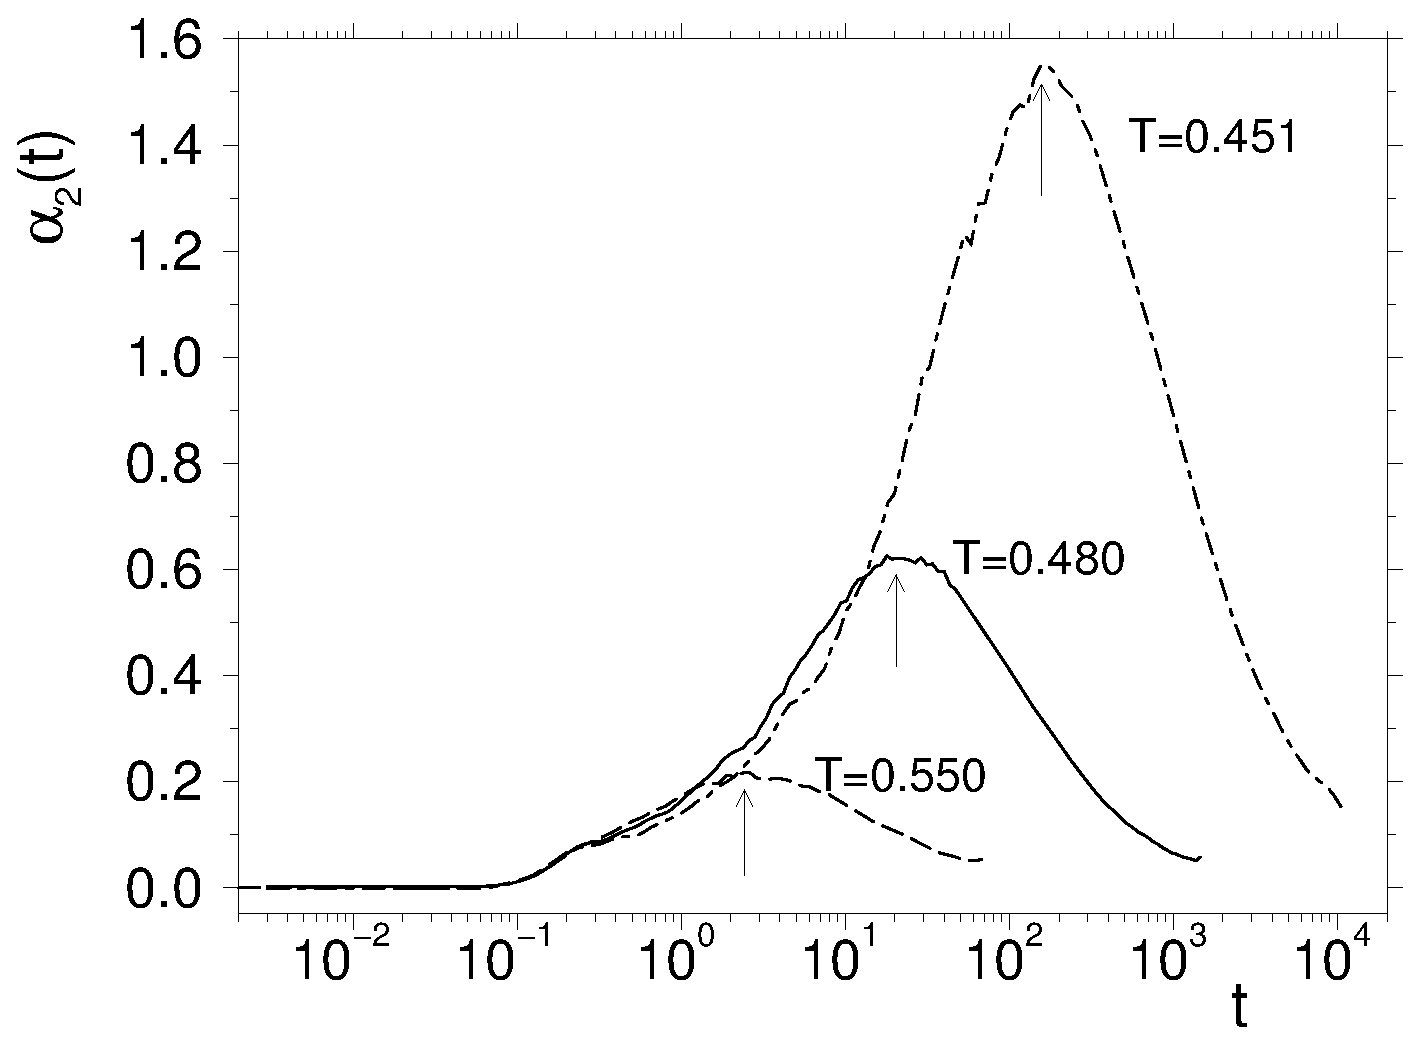
\includegraphics[width=0.5\textwidth]{ngp_kob}}
	\subfloat
		[Time and temperature dependence of the dynamical correlation length $\xi_4(t)$. From~\citep{Lacevic2003}.]
		{\label{fig:xi4}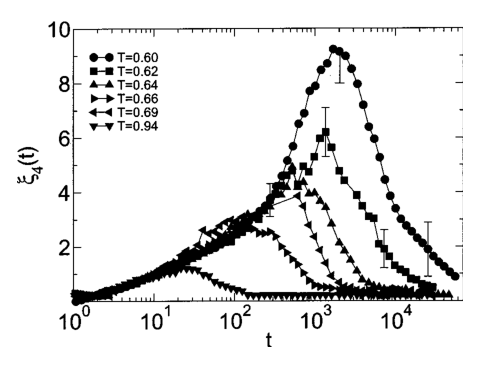
\includegraphics[width=0.5\textwidth]{xi4_lacevic}}
	\caption{Non-gaussianity of the dynamics and corresponding dynamical correlation length in a binary Lennard-Jones system.}
\end{figure}


The non-gaussianity of the displacements translates into a distribution of time scales for the $\alpha$ relaxation. Indeed, the long time part of the self \ac{ISF} is not a single exponential. It is rather well fitted by the Kohlraush-Williams-Watts~\citep{Kohlrausch1847, Williams1970} stretched exponential form $A \exp{\left[ -\left( t/\tau_\alpha \right)^\beta\right] }$ with $\beta<1$ the stretching exponent and $A$ the height of the plateau, also called the Debye-Waller factor. As a whole, the self \ac{ISF} can be fitted as:
\begin{equation}
	F_s(q,t) \sim (1-A) \exp{\left[-\frac{t}{\tau_\beta}\right] } + A \exp{\left[ -\left( \frac{t}{\tau_\alpha} \right)^\beta\right] }
	\label{eq:streched_exp_2steps}
\end{equation}

With this definition, the \ac{NGP} reaches its maximum at a time scale a few times smaller than $\tau_\alpha$. Then, the value of the self \ac{ISF} approximatively corresponds to the Debye-Waller factor.

\subsection{Dynamic Heterogeneities}
\label{sec:dynhet}

\begin{figure}
	\centering
	\subfloat
		[Dynamic heterogeneities in a 2D supercooled liquid simulation. Plot of the end-to-end particle displacement vectors. From~\citep{Perera1999}]
		{\label{fig:dh_perera}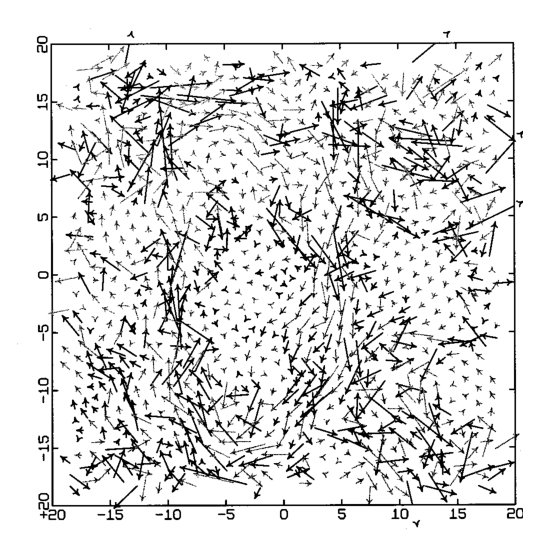
\includegraphics[width=0.5\textwidth]{dh_perera}}
	\subfloat
		[Dynamic heterogeneities in hard sphere supercooled liquid experiments. The locations of the fastest particles (large spheres) and the other particles (smaller spheres).  From~\citep{weeks2000}]
		{\label{fig:dh_weeks}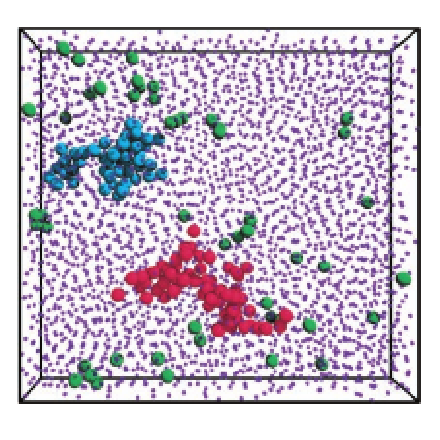
\includegraphics[width=0.5\textwidth]{dh_weeks}}
	\caption{Visualisation of dynamic heterogeneities. When calculated according to the appropriate time scale $t^{dh}$, the displacements of the particles show heterogeneities in space. In \subref{fig:dh_weeks} the particles all have the same physical size, which is the size of the large spheres.}
	\label{fig:dynhet}
\end{figure}

As we said at the end of \SectionRef{sec:cage}, the relaxation in a supercooled liquid is not a single-particle process; it involves a group of particles that have to rearrange cooperatively. This notion articulates with the non-gaussianity of the dynamic to give the notion of dynamic heterogeneities: groups of particles rearrange cooperatively many times which yields a high mobility for these particles, when other regions of the system are not rearranging implying that the particles there are localised~\citep{Kob1997, Donati1998, Donati1999, kegel2000swe, Perera1999, weeks2000, weeks2002pcr}.

The dynamic heterogeneities are best observed (see \FigureRef{fig:dynhet}) when calculating the value of dynamical functions at the maximum of the \ac{NGP}. We note the time scale of this maximum $t^{dh}$. Once again, we need two times (or a difference of times) to describe the physics of the system. Even more interesting is the size of the dynamic heterogeneities that is increasing when approaching the glass transition (see \FigureRef{fig:xi4}).


\subsection{How to define a dynamical length scale}
\label{sec:dyn_length}
To define the characteristic length scale of the dynamic heterogeneities, \citet{Donati1999} thought about correlating in space the displacements $\Delta r_i(t) = \vec{r}_i(t)-\vec{r}_i(0)$ or more precisely, the fluctuations of the norm of the displacements $\delta u_i(t) = \Delta r_i(t) - \left\langle \Delta r_i(t) \right\rangle$. The mobility-mobility spatial correlation function is defined as:
\begin{equation}
	\mathcal{G}_{u(t)}(r) \equiv \mathcal{G}_u(r,t) \equiv \frac{
		\left\langle \sum_{i,j}{\delta u_i(t) \delta u_j(t) \delta(r_{ij} -r)} \right\rangle 
	}{
		\left\langle \sum_{i,j}{\delta(r_{ij} -r)} \right\rangle
	}
	\label{eq:mobility_correl}
\end{equation}

Note that for $r=0$ \EquationRef{eq:mobility_correl} boils down to the \ac{MSD} (\EquationRef{eq:msd}). $\mathcal{G}_u(t,r)$ informs us about the spatial fluctuations of the \ac{MSD}. The four-point correlation function that corresponds in the same way to the spatial fluctuations of the \ac{ISF}~\citep{Lacevic2003} is 
\begin{equation}
	 \mathcal{G}_4(r, t) \equiv 
	 	\left\langle \delta\rho(0,0)\delta\rho(0,t) \delta\rho(r,0)\delta\rho(r,t) \right\rangle 
	 	- \left\langle \delta\rho(0,0)\delta\rho(0,t) \right\rangle 
	 		\left\langle \delta\rho(r,0)\delta\rho(r,t) \right\rangle
	 \label{eq:four_point_correl}
\end{equation}

The name "four-point correlation function" stands for the $4$ points needed to defined such a function: $r_i(t_0)$, $r_i(t_0+t)$, $r_j(t_0)$ and $r_j(t_0+t)$. We can define a susceptibility for each of these functions,
\begin{align}
	\chi_u =& \int{dr \mathcal{G}_u(t,r)} \label{eq:dynamic_susc}\\
	\chi_4 =& \int{dr \mathcal{G}_4(t,r)} \label{eq:chi4}
\end{align}
and a correlation length $\xi_u(t)$, $\xi_4(t)$ from the decay of the correlation function. The largest susceptibility and the longer correlation length can be obtained for $t=t^{dh}$ (see \FigureRef{fig:xi4}). Thus from now on if $t$ is omitted in a four-point observable, it means $t=t^{dh}$.


\section{A static cause to dynamic heterogeneities?}
\label{sec:static_cause}

\subsection{The quest for a static length scale}
\label{sec:static_length}

We saw in \SectionRef{sec:X+glass} that the usual static correlation function where not changing significantly when approaching the glass transition. Nothing spectacular happens in the positional order of the system when simultaneously its dynamics slows down by many orders of magnitude. In critical phenomena a static correlation length (the characteristic size of the critical fluctuations) diverges, which are responsible for the dramatic slowing down of the system: the larger, the slower. No diverging static correlation length could be found for decades in glass forming liquids.

In \SectionRef{sec:dynhet} and \SectionRef{sec:dyn_length} we saw that a dynamic correlation length can be defined corresponding to dynamic heterogeneities in the system. If we could find a static cause to the dynamic heterogeneities, its length scale is likely to increase in the same way as the dynamic correlation length, achieving the quest for a static length diverging at the glass transition.

In this section, we will review the body of evidence that points toward the existence of a static cause, whatever it is, to the dynamic heterogeneities.

\subsection{Dynamic propensity}
\label{sec:propensity}

\begin{figure}
	\centering
	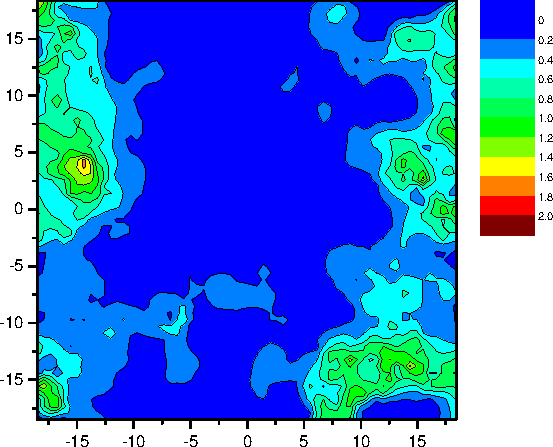
\includegraphics[width=0.8\textwidth]{propensity}
	\caption{Dynamic propensity map of a 2D soft disk simulation. From~\citep{Widmer-Cooper2005}}
	\label{fig:propensity}
\end{figure}

It is quite natural to think that a rearrangement at a given place will trigger other rearrangements nearby because it offers new possibilities of motion. It is thus difficult to disentangle the influence of the static structure from the the consequences of previous dynamical events. To address this point, \citet{Widmer-Cooper2005} introduced the iso-configurational ensemble and the dynamic propensity.

The iso-configurational ensemble is a simulation trick to get rid of the influence of the initial dynamics. \citet{Widmer-Cooper2005} ran $M$ simulations with the same starting configuration but with momenta assigned randomly from the appropriate Maxwell–Boltzmann distribution. If $M$ is large enough, the average over those runs of any observable should be depending only on the initial configuration. If the iso-configurational averaged observable is spatially homogeneous, then this observable do not depend on the initial configuration.

\citet{Widmer-Cooper2005} named \emph{dynamic propensity} the iso-configurational average of the square displacement, because it does not correspond to the actual squared displacement of the particle in any particular run but, rather, reflects the particle's propensity for displacement. As shown in \FigureRef{fig:propensity}, the propensity is heterogeneous, so the structure can predict the propensity. Subsequent works focused mainly on the predictability of the propensity by the structure~\citep{Widmer-Cooper2007, Matharoo2006, Coslovich2006, Appignanesi2006, RodriguezFris2007, Hedges2007, Downton2007}.

\subsection{Predicting the dynamics}

\citet{Berthier2007} showed that the propensity was in fact a poor predictor of the dynamics at the particle level. In particular, the distinction between fast and slow particles is no longer apparent after iso-configurational average. So the link between structure and dynamics \latin{via} the propensity seems to be broken. 

However the same authors show that at larger scales the dynamic propensity predicts well the size and the geometry of the dynamic heterogeneities. While it is not possible to use the structure to predict whether a given particle will be fast or slow in a single run, it is possible to tell if it belongs to a fast or slow region.

In particular, the structure should be able to predict the diverging size of the dynamic heterogeneities. So the quest for a static diverging length scale is not vain.

\subsection{What sort of static cause?}

Even if we know that the initial positions of the particles plays a role in the dynamic heterogeneities, the precise static features that control the dynamics are still to be determined. Various attempts have been made in this direction, considering the elastic properties~\citep{Brito2006, Widmer-Cooper2008, Tsamados2009}, the configurational entropy~\citep{adam1965tdr, Kirkpatrick1987a, Kirkpatrick1987, kirkpatrick1989scd}, or through the idea of a rough energy landscape~\citep{Stillinger1984}. These approaches often focus on the rearranging regions, trying to understand why, when and how they rearrange.

Another line of thought is to focus on the slow regions and understand why they are not rearranging. After all, the specificity of the glass transition is a slowing down, not that particles move. The notion that some stable structures form in the supercooled liquid emerges quite naturally. However, the term "structure" has to be defined properly. We said in \SectionRef{sec:X+glass} that the usual definition of order, well adapted to distinguish between a long-range positionally ordered crystal and the disordered high temperature liquid, was not sufficient to detect the onset of the glass transition. The structure that may exist in supercooled liquid must then be local or medium-ranged and not detectable by the usual two-point density correlation methods.

The frustration-based approach~\citep{tarjus2005fba} postulates the existence of a local order in any liquid, order that cannot tile the whole space, for instance the $5$-fold symmetry. Without this geometric frustration, the order would fill space and be at even lower energy than the crystal. The partial ordering despite frustration would be the origin of the slowing down.

\begin{figure}
	\centering
	\subfloat[$\psi_6$]{\label{fig:kawa_nm_psi6}\def\svgwidth{0.3\textwidth}\input{kawa_nm_psi6.pdf_tex}}
	\subfloat[$\Delta r^2$]{\label{fig:kawa_nm_msd}\def\svgwidth{0.3\textwidth}\input{kawa_nm_msd.pdf_tex}}
	\subfloat[$Q_6$]{\label{fig:kawa_nm_3d}\def\svgwidth{0.3\textwidth}\input{kawa_nm_3d.pdf_tex}}
	\caption{\subref{fig:kawa_nm_psi6} fluctuations of the crystal-like bond order parameter in polydisperse quasi hard disks simulations and \subref{fig:kawa_nm_msd} the corresponding dynamic heterogeneities. \subref{fig:kawa_nm_3d} Same as \subref{fig:kawa_nm_psi6} in 3D, but the low order particles are not shown for clarity. From~\citep{tanaka2010critical}.}.
	\label{fig:kawa_nm}
\end{figure}

Tanaka~\cite{tanaka1999top,Tanaka1999} noticed that the avoided crystallisation should not be forgotten in the supercooled branch. By definition a supercooled liquid is metastable to a crystal and the underlying tendency to crystalline ordering must be important. The avoidance of crystallisation, the dynamical arrest and the fragility can be all linked by using two order parameters that account respectively for the tendency toward global ordering (crystallisation) and the formation of locally favoured structures incompatible with the crystal symmetry. The term "frustration" is also used in the two order parameter model, but it is related to the frustation on the way to crystallisation~\citep{tanaka2005top, Tanaka20053371, Tanaka20053385, Shintani2006}, not to a type of order intrinsically frustration by the geometry of space.

Tanaka and co-workers~\citep{kawasaki2007cbd, Shintani2006, watanabe2008, Kawasaki2010} showed that in various systems (simulations and 2D granular matter experiments) the fluctuations of the local crystalline order are closely related to dynamic heterogeneities (see \FigureRef{fig:kawa_nm}). Moreover, the length scale of these fluctuations show an Ising-like power-law divergence toward the glass transition point~\citep{tanaka2010critical}. These results suggest a far more direct link than thought before between the glass transition and critical phenomena. Indeed, the glass transition may be a new type of critical phenomenon where a structural order parameter is directly linked to slowness. Furthermore, this structural ordering accompanies little change in density, which explains why it has not been detected by the static structure factor so far.

The present work is based on these results and try to test and extend them in 3D by experiments.


\section{Hard spheres and colloids}
\label{sec:HS-colloids}

The experimental systems that allow to to probe directly their local structure are few. The present section introduces one of them that is investigated in this thesis: colloidal hard spheres.

\subsection{Crystallisation and glass transition}

\begin{figure}
	\centering
	\def\svgwidth{0.9\textwidth}
   	\input{phase_diagram.pdf_tex}
	
	\caption{Behaviour of almost identical hard spheres upon increasing volume fraction from 0.4 (usual liquid) to 0.74 (close packing). Top: Equilibrium phase diagram for the monodisperse system. Bottom: metastable branch with respect to the avoided crystallisation for $6\%$ polydispersity.}
	\label{fig:HS_phase_diagram}
\end{figure}

Hard spheres are defined as impenetrable spheres. Apart from this no overlap condition, they have neither repulsion nor attraction between them, so no potential energy. This very simple definition makes this theoretical object a cornerstone of statistical mechanics, and it has been subjected to an exceptional degree of interest, to the extent that hard spheres form one of the best understood systems of condensed matter. In particular, a first order fluid-to-crystal freezing transition of hard spheres was discovered more than 50 years ago in the early computer experiments of \citet{wood1957} and \citet{alder1957}.

Hard sphere crystallization is puzzling. Why would a system without potential energy, driven only by entropy, prefer order to disorder? The answer was suggested by \citet{hoover1958}: a globally ordered configuration allows more vibration of each particle than a disordered configuration. In terms of \EquationRef{eq:config_vib}, the crystallisation decrease the configurational entropy $S_c$ but increases the vibrational entropy $S_{vib}$. At high enough density $|\Delta S_c|<|\Delta S_{vib}|$ so the entropy paradoxically increases upon (global) ordering.

Not long after this discovery, drawing on their own free-volume theories and sphere packing experiments~\citep{Scott1960, Bernal1960}, \citet{Cohen1959, Cohen1964} suggested that compressing an assembly of hard spheres fast enough to by-pass crystallization should result in a metastable, amorphous, solid "glass" state. In 1986, experiments by \citet{pusey1986} on suspensions of colloidal particles that interact via a steep repulsive potential observed both the freezing transition and, at higher concentrations, glass formation.

\subsection{Equations of state}
\label{sec:eos}

In the case of the single component hard sphere fluid, the osmotic pressure is well-approximated by the Carnahan-Starling \ac{EOS}~\citep{carnahan1969},
\begin{equation}
\frac{PV}{N k_B T}=\frac{1 + \phi + \phi^2 - \phi^3}{(1 - \phi)^3}
\label{eq:CS}
\end{equation}
where $P$ is pressure, $V$ is volume, $N$ is the number of particles within $V$ and $\phi$ is the volume fraction defined as 
\begin{equation}
	\phi \equiv N \frac{\pi\sigma^3}{6 V}
	\label{eq:vf_mono}
\end{equation}
where $\sigma$ is the hard core diameter. The volume fraction is the only control parameter of the phase behaviour of monodisperse hard spheres. When comparing between hard spheres and systems having a potential energy, one may think about the volume fraction as an inverse temperature: increasing the volume fraction is somewhat equivalent as cooling a thermal system. At $\phi=\phi_m \equiv 0.4954$ monodisperse hard spheres freeze and at $\phi=\phi_X \equiv 0.5478$ they melt. At higher volume fractions one finds a kinetic glass transition volume fraction $\phi_g$ before reaching an theoretical ideal glass transition at $\phi_0$. In general, all the relations that we presented in the previous sections of this chapter can be adapter to the case of hard spheres by changing $T$ in $1/\phi$.

The osmotic pressure of the single component hard sphere crystal is well approximated by the form given by \citet{hall1972}.
\begin{equation}
\frac{PV}{N k_B T} = \frac{
1 + \phi + \phi^2 - 0.67825 \phi^3 - \phi^4 - 0.5 \phi^5 - 6.028 e^{\phi\epsilon(7.9-3.9\phi\epsilon)}\phi^6
}{
1 - 3 \phi + 3 \phi^2 - 1.04305 \phi^3
}
\label{eq:Hall}
\end{equation}
where $\epsilon=\phi_{cp}/\phi -1$ quantifies the distance to the close packing volume fraction $\phi_{cp} = \pi\sqrt{2}/6 \simeq 0.74$. The parametrization given by \citet{Young1979} is also often used for its simplicity even though it deviates from Hall's for small $\phi$.
\begin{equation}
\frac{PV}{Nk_{B}T} = \frac{3}{\epsilon} + 2.566 + 0.55 \epsilon - 1.19 \epsilon^2 + 5.95 \epsilon^3
\label{eq:Alder}
\end{equation}

\subsection{Colloidal hard spheres}
\label{sec:colloidalHS}
In addition to their fundamental simplicity, hard spheres have been very closely approximated experimentally using colloidal dispersions. \ac{DLVO} theory suggests that the stability of a colloidal dispersion depends on the sum of the attraction and repulsion potential (\FigureRef{fig:DLVO-a}). the attractive component is usually due to short ranged van der Waals forces. It causes irreversible aggregation of the colloids. The repulsive interaction potential is long ranged and due to the electrostatic double layer made of the charge on the colloids and of the counter ions in the solvent. The range of this repulsive potential is the Debye length. Adding salts to the solvent is diminishing the Debye length. In aqueous media, it will easily destabilize the colloidal dispersions, making it fall into the primary minimum due to the van der Waals interaction. In non-aqueous media, the dielectric constant is weaker so the Debye length is never short enough to have an unstable colloidal dispersion. On the contrary, the double layer energy can be enforced by adding salts to the solvent, stabilizing the suspension.

\begin{figure}
	\centering
	\subfloat[Free energy variation function
of the particle separation.]{\label{fig:DLVO-a}\def\svgwidth{0.4\textwidth}\input{dlvo_theory_1.pdf_tex}}
	\subfloat[In the case of highly charged solutions,
a second minimum appears.]{\def\svgwidth{0.4\textwidth}\input{dlvo_theory_2.pdf_tex}}
	\caption{\acl{DLVO} theory.}
	\label{fig:DLVO-theory}
\end{figure}

The key to approximate hard spheres with almost uncharged colloidal dispersions is the steric stabilization~\citep{pusey1986}. Polymers are adsorbed or even bind to the colloids to keep their surface further apart than the van der Waals attraction range, preventing aggregation.

\subsection{Polydispersity}
\label{sec:poly}
The usual way to avoid crystallisation of spherical particles is to mix two or more types of particles, like in the well known Kob-Anderson binary mixture of Lennard-Jones particles~\citep{kob1995tmc}. Colloids naturally present a distribution of sizes, often approximated as Gaussian. Monodisperse colloids are impossible but can be approximated as close as $3\%$ polydispersity. 

This experimental constrains motivated investigations about the effect of polydispersity on the phase behaviour of hard spheres by experiments~\citep{pusey1986, pusey}, computer simulations~\citep{Dickinson1985, Bolhuis1996, Phan1998}, density functional theories~\citep{Barrat1986, McRae1988}, and simplified analytical theories~\citep{Barrat1986, Pusey1987, McRae1988, Bartlett1997, Sear1998, bartlett1999, Xu2003}. These studies have revealed that, compared to the monodisperse case, polydispersity causes several qualitatively new phenomena. 

It is intuitively clear~\citep{Pusey1987} that significant diameter polydispersity should destabilize the crystal phase, because it is difficult to accommodate a range of diameters in a lattice structure. Polydispersity induces geometrical frustration against crystallisation. Experiments indeed show that crystallization is suppressed above a terminal polydispersity of $\Delta_t \simeq 12\%$~\citep{pusey1986, pusey}. Theoretical work suggested that this arises from a progressive narrowing of the fluid-solid coexistence region with increasing $\Delta$, with the phase boundaries meeting at $\Delta_t$~\citep{McRae1988, Bartlett1997} in a point of equal concentration~\citep{bartlett1999}. \citet{Fasolo2003} refined the previous determinations of $\Delta_t$ by taking into account the fractionation into several solid phases that occurs at sufficiently large polydispersity. They found $\Delta_t \simeq 7\%$.

Kawasaki \latin{et al.} showed in simulation that polydispersity also affects the fragility of (almost) hard disks~\citep{kawasaki2007cbd} and (almost) hard spheres~\citep{Kawasaki2010}. Higher polydispersity induces stronger glass. Frustration against crystallization has been shown to decrease fragility in various other systems~\citep{tarjus2005fba, Shintani2006, molinero2006tts, Coslovich2007, watanabe2008, tanaka2010critical}. So the polydispersity~$\Delta$, which controls the degree of frustration against crystallization, governs not only glass-forming ability, but also the fragility, or the glass transition behaviour.

\subsection{Simulation data}
\label{sec:sim_kawa}

In this thesis we will sometimes re-analyse the simulations ran by Takeshi Kawasaki~\citep{tanaka2010critical, Kawasaki2010}.

From his data, we used the closest from our experiments that were available: \ac{BD} simulations of hard-sphere-like particles interacting with the \ac{WCA} repulsive potential
\begin{equation}
	U_{jk}(r) = \left\{\begin{array}{l l}
  		4\epsilon\left[ \left( \frac{\sigma_{jk}}{r}\right)^{12} - \left( \frac{\sigma_{jk}}{r}\right)^{6} +\frac{1}{4}\right]  & \quad \text{for $r<2^\frac{1}{6} \sigma_{jk}$}\\
  		0 & \quad \text{otherwise}
  	\end{array} \right.
	\label{eq:WCA}
\end{equation}
where $\epsilon$ gives the energy scale, $\sigma_{jk} = (\sigma_j + \sigma_k)/2$. The effective diameter of the particle is defined where the potential energy becomes equal to the thermal energy:
\begin{equation}
	U(\sigma_{eff}) = k_B T
\end{equation}
where $k_B$ is the Boltzmann constant. The temperature is fixed at $k_B T/\epsilon = 0.025$. The volume fraction is calculated using $\sigma_{eff} = 1.095\sigma$.

Unless mentioned otherwise, the size polydispersity is Gaussian with $\Delta=6\%$.

\section{Aim and plan}

Our goal in this thesis is to investigate the structures appearing in a hard sphere liquid upon supercooling and to make the link between some of these structures and the dynamic heterogeneities. Thus, we may be able to describe the glass transition by the mean of a static (structural) characteristic size that would diverge at an ideal glass transition volume fraction.

The body of this thesis is divided into two parts. In the first one we explain the methods, original or from the literature, that are used in the second part to output results about the structure of our system (\ChapterRef{ch:structure}), its dynamics and the relationship between the two (\ChapterRef{ch:results_dynamics}). The closely related matter of crystallisation will be discussed in \ChapterRef{ch:crystallisation}.